%%%%%%%%% Part III %%%%%%%%%

\par \noindent To assess the question about the welfare gains associated with moving
from incomplete to complete markets, compute \textbf{\color{red} consumption equivalents} using
the following formulas. For each $(a,s)$ we compute $\lambda(a,s)$ such that
\begin{eqnarray}
    W &= &\E\left[ \sum_{t=0}^\infty \beta^t
    \frac{\big[(1+ {\color{red} \lambda(a,s) })c_t(a,s)\big]^{1-\alpha}-1}{1-\alpha}
    \,\bigg| (a,s)\right] \\[1em]
    &= &(1+\lambda(a,s))^{1-\alpha}
        {\color{blue} \E\left[ \sum_{t=0}^\infty \beta^t
                \frac{c_t(a,s)^{1-\alpha}}{1-\alpha}\right]}
    - \frac{1}{(1-\alpha)(1-\beta)} \\[1em]
    &=& (1+\lambda(a,s))^{1-\alpha}
    \left[ v(a,s) + \frac{1}{(1-\alpha)(1-\beta)} \right]
    - \frac{1}{(1-\alpha)(1-\beta)}, \\[1em]
    \Longleftrightarrow \quad {\color{red} \lambda(a,s) } & = & \left[
        \frac{ W + \dfrac{1}{(1-\alpha)(1-\beta)} }
        { v(a,s) + \dfrac{1}{(1-\alpha)(1-\beta)} }
        \right]^{1/(1-\alpha)} - 1
\end{eqnarray} where $ v(a,s)$ is the value function from the incomplete markets economy.

%%%%% Exercise 3.1
\begin{framedexercise}[Consumption equivalents $\lambda(a,s)$]
    Plot $\lambda(a,s)$ across $a$ for both $s= e$ and $s= u$ in the same graph.
\end{framedexercise}

\begin{solution} Consumption equivalents $\lambda(a,s)$ are plotted in Figure \ref{fig:CE}. \qed
    %
    \begin{figure}[H]
        \centering
        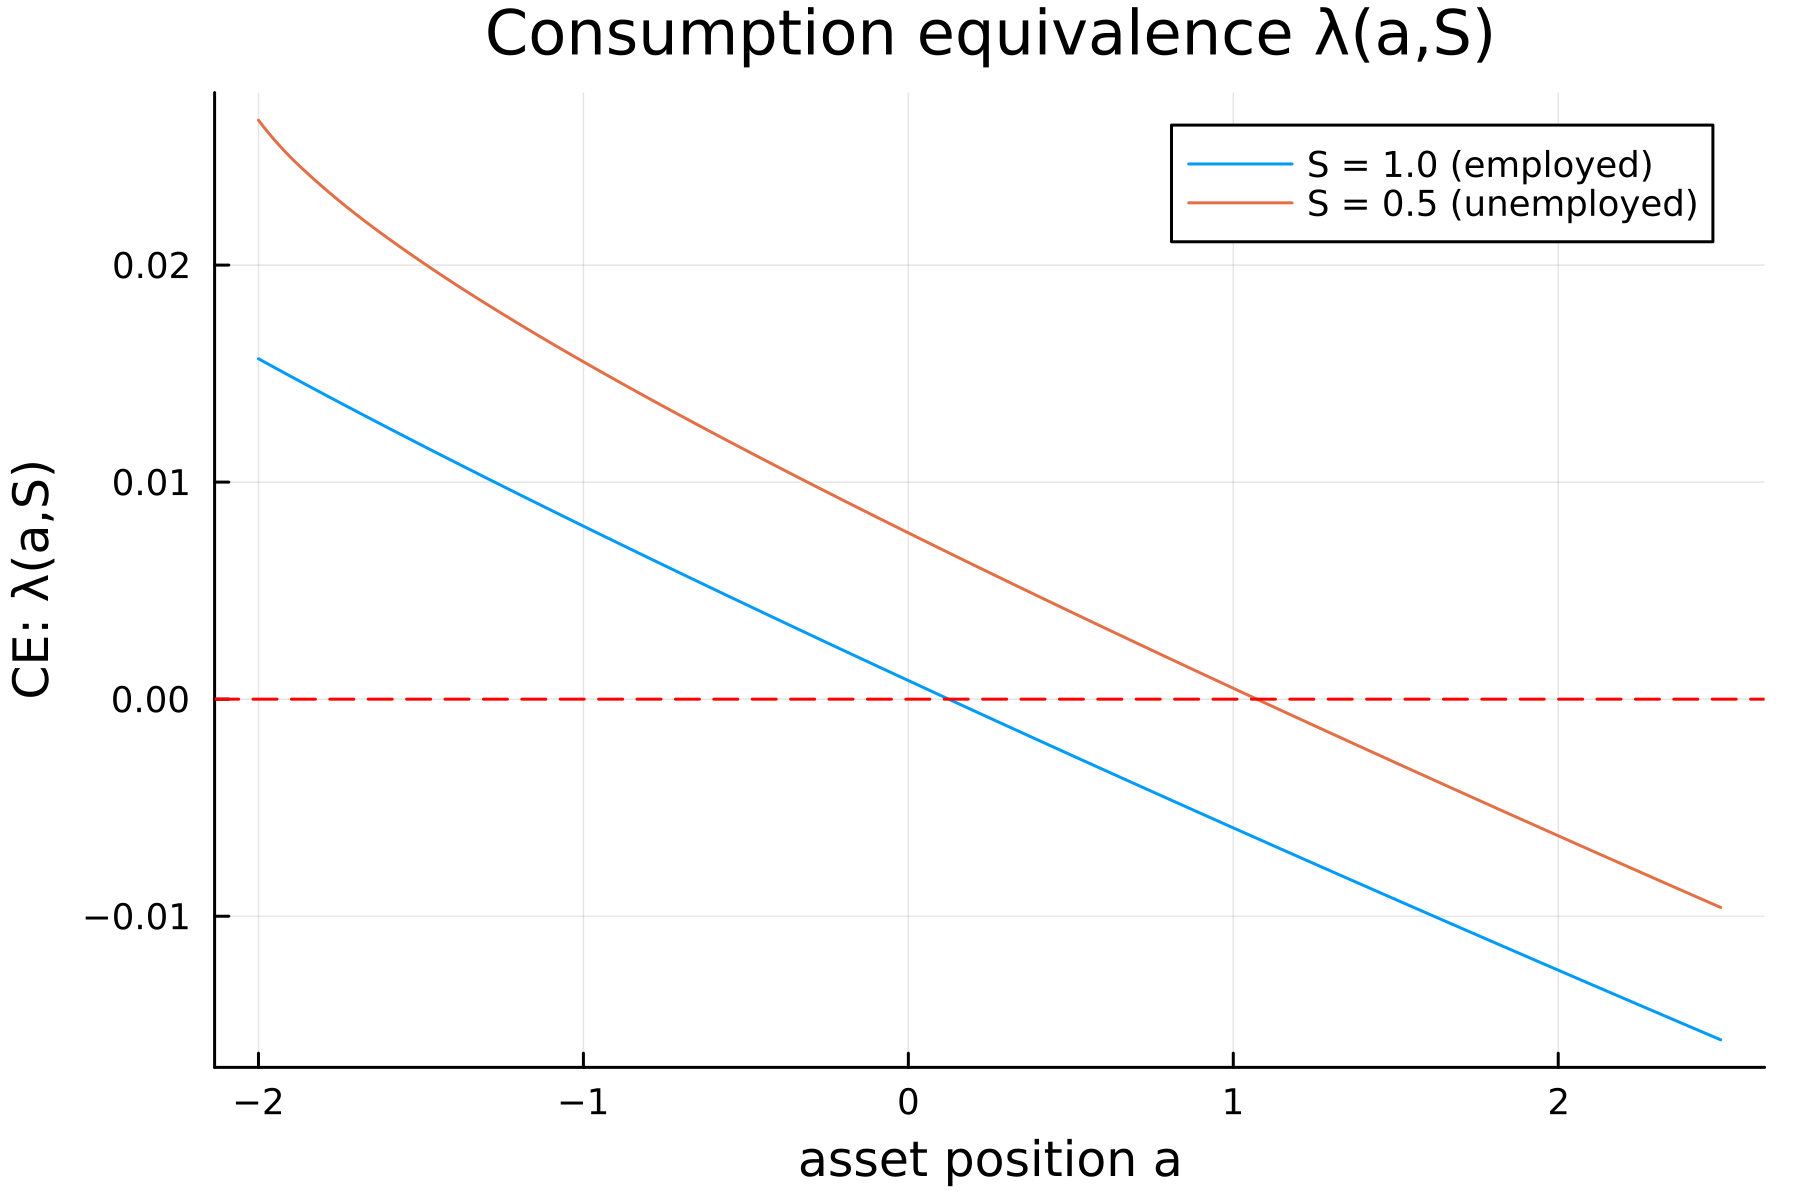
\includegraphics[width=0.6\textwidth, angle=0]
        {5 Consumption_Equivalence.png}
        \caption{Consumption Equivalents by Asset and Employment states}
        \label{fig:CE}
    \end{figure}
\end{solution}

\newpage
%%%%% Exercise 3.2
\begin{framedexercise}[Welfare in two markets and welfare gains/losses] The welfare in complete market (henceforce $W^{FB}$) is:
    \begin{eqnarray}
        W^{FB} & = & \E\left[ \sum_{t=0}^\infty \beta^t
            \frac{(c^{FB})^{1-\alpha}-1}{1-\alpha} \right] \\
        & \xRightarrow[\text{\scriptsize stationary}]{\text{\scriptsize $c^{FB}$}} & \sum_{t=0}^\infty \beta^t
        \frac{(c^{FB})^{1-\alpha}-1}{1-\alpha} = \frac{(c^{FB})^{1-\alpha}-1}{(1-\alpha)(1-\beta)}.
    \end{eqnarray}
    The economywide welfare gain (or loss) from switching back to complete market is  given by
    \begin{eqnarray}
        WG = \sum_{(a,s) \in A \times S} \lambda(a,s)\mu(a,s).
    \end{eqnarray} Then, \begin{itemize}
        \item[\circled{1}] What is $W^{FB}$?
        \item[\circled{2}] What is $W^{INC}$, where
              \begin{eqnarray}
                  W^{INC} = \sum_{(a,s) \in A \times \mathcal{S}} \mu(a,s) v(a,s)
              \end{eqnarray}
        \item[\circled{3}] What is $WG$, the welfare gain (or loss) from switching back to complete markets?
    \end{itemize}
\end{framedexercise}

\begin{solution}
    From my Julia terminal, $W^{FB}$ (rounded to 5 digits) is $-4.25252$.
    $W^{INC}$ (rounded to 5 digits) is $-4.45153$. This aligns to class slides,
    \textit{``Aggregate welfare is higher in the complete markets economy than
        the incomplete markets economy (no surprise)''}.
    The welfare gain of switching to complete markets (rounded to 5 digits) is $0.00134$. \qed
\end{solution}

%%%%%% Exercise 3.3
\begin{framedexercise}[Switching back or not] What fraction of the population would favor changing to complete markets?
    That is, \begin{eqnarray}
        \sum_{(a,s) \in A \times S} \mathbb{1}\{\lambda(a,s) > 0\} \mu(a,s).
    \end{eqnarray}
\end{framedexercise}

\begin{solution}
    From my Julia terminal, the fraction of agents that favor switching
    to complete markets (rounded to 5 digits) is $0.54145$.
    This is highlighted by the $\lambda(a,s) \geq 0$ (i.e., above red dashed line) in Figure \ref{fig:CE}. \qed
\end{solution}